% -----------------------------------
% -----------------------------------
% abnTeX2: Normas ABNT NBR 14724:2011 + sugestões FGV/EMAp. 

% Autor: Lauro César Araujo
% Adaptações EMAp: Lucas Machado Moschen 
% Copyright 2012-2018 by abnTeX2 group at http://www.abntex.net.br/ 

%% This work may be distributed and/or modified under the
%% conditions of the LaTeX Project Public License, either version 1.3
%% of this license or (at your option) any later version.
%% The latest version of this license is in
%%   http://www.latex-project.org/lppl.txt
%% and version 1.3 or later is part of all distributions of LaTeX
%% version 2005/12/01 or later.
% ----------------------------------
% ----------------------------------
\documentclass[
	% -- opções da classe memoir --
	12pt,				% tamanho da fonte
	%openright,			% capítulos começam em página ímpar (insere página vazia caso preciso)
	oneside,			% para impressão em recto e verso. Oposto a oneside
	a4paper,			% tamanho do papel. 
	% -- opções da classe abntex2 --
	%chapter=TITLE,		% títulos de capítulos convertidos em letras maiúsculas
	%section=TITLE,		% títulos de seções convertidos em letras maiúsculas
	%subsection=TITLE,	% títulos de subseções convertidos em letras maiúsculas
	%subsubsection=TITLE,% títulos de subsubseções convertidos em letras maiúsculas
	% -- opções do pacote babel --
	english,			% idioma para inglês
	brazil				% idioma para português
	]{abntex2}

%------------------------------------------------
%-------------- Pacotes necessários -------------
%------------------------------------------------

% Escrita 
\usepackage[T1]{fontenc}
\usepackage[utf8]{inputenc}
\usepackage{lmodern}
\usepackage{microtype} % para melhorias de justificação
\usepackage{indentfirst}

\renewcommand{\ABNTEXchapterfont}{\fontfamily{ptm}\fontseries{b}\selectfont}

% Gráficos 
\usepackage{color}
\usepackage{caption}
\usepackage{subcaption}
\usepackage{graphicx}
\graphicspath{{../../images/}}

% Matemáticos 
\usepackage{amsthm, amssymb, amsmath, mathtools}

% Outros 
\usepackage{listings}
\renewcommand{\lstlistingname}{Código}
\renewcommand{\lstlistlistingname}{Lista de códigos}
\lstset{basicstyle=\ttfamily\footnotesize,breaklines=true, numbers=left,
inputencoding=utf8, extendedchars=true, frame=single,
literate=%
        {é}{{\'{e}}}1
        {è}{{\`{e}}}1
        {ê}{{\^{e}}}1
        {ë}{{\¨{e}}}1
        {É}{{\'{E}}}1
        {Ê}{{\^{E}}}1
        {û}{{\^{u}}}1
        {ù}{{\`{u}}}1
        {ú}{{\'{u}}}1
        {â}{{\^{a}}}1
        {à}{{\`{a}}}1
        {á}{{\'{a}}}1
        {ã}{{\~{a}}}1
        {Á}{{\'{A}}}1
        {Â}{{\^{A}}}1
        {Ã}{{\~{A}}}1
        {ç}{{\c{c}}}1
        {Ç}{{\c{C}}}1
        {õ}{{\~{o}}}1
        {ó}{{\'{o}}}1
        {ô}{{\^{o}}}1
        {Õ}{{\~{O}}}1
        {Ó}{{\'{O}}}1
        {Ô}{{\^{O}}}1
        {î}{{\^{i}}}1
        {Î}{{\^{I}}}1
        {í}{{\'{i}}}1
        {Í}{{\~{Í}}}1
}

% Citações 
%\usepackage[brazilian,hyperpageref]{backref}
%\usepackage[alf]{abntex2cite}	% Citações padrão ABNT
\usepackage[style=abnt]{biblatex}
\addbibresource{biblio.bib}  

% \renewcommand{\backrefpagesname}{Citado na(s) página(s):~}
% % Texto padrão antes do número das páginas
% \renewcommand{\backref}{}
% % Define os textos da citação
% \renewcommand*{\backrefalt}[4]{
% 	\ifcase #1 %
% 		Nenhuma citação no texto.%
% 	\or
% 		Citado na página #2.%
% 	\else
% 		Citado #1 vezes nas páginas #2.%
% 	\fi}%
% ---

%----------------------------------------
%------- Capa e Folha de Rosto ----------
%----------------------------------------

\newcommand\subtitulo[1]{\def\@subtitulo{#1}}
\newcommand{\imprimirsubtitulo}{\@subtitulo}

\renewcommand{\imprimircapa}{%
	\begin{capa}%
	\center
		\ABNTEXchapterfont\Large \MakeUppercase{\imprimirinstituicao}
		\\\vspace*{4cm}
		{\ABNTEXchapterfont\large \MakeUppercase{\imprimirautor}}
		\vfill
		\begin{center}
		\ABNTEXchapterfont\large\MakeUppercase{\imprimirtitulo}\normalfont\MakeUppercase{:
		\imprimirsubtitulo}
		\end{center}
		\vfill
		\normalfont\large\imprimirlocal
		\\\normalfont\large\imprimirdata
		\vspace*{1cm}
	\end{capa}
}

\makeatletter
\renewcommand{\folhaderostocontent}{
  \begin{center}

    %\vspace*{1cm}
    {\ABNTEXchapterfont\large\MakeUppercase{\imprimirautor}}
	
    \vspace*{\fill}\vspace*{\fill}
    \begin{center}
      \ABNTEXchapterfont\bfseries\large\MakeUppercase{\imprimirtitulo}\normalfont\MakeUppercase{:
      \imprimirsubtitulo}
    \end{center}
    \vspace*{\fill}
	
    \abntex@ifnotempty{\imprimirpreambulo}{%
      \hspace{7.5cm}
      \begin{minipage}{.5\textwidth}
      	\SingleSpacing
         \imprimirpreambulo
         \\\\
         Orientador: \imprimirorientador
       \end{minipage}%
       \vspace*{\fill}
    }%

    % {\large\imprimirorientadorRotulo~\imprimirorientador\par}
    % \abntex@ifnotempty{\imprimircoorientador}{%
    %    {\large\imprimircoorientadorRotulo~\imprimircoorientador}%
    % }%
    \vspace*{\fill}

    {\large\imprimirlocal}
    \par
    {\large\imprimirdata}
    \vspace*{1cm}

  \end{center}
}
\makeatother

\titulo{Geodesic Tracing}
\subtitulo{Visualização de curvas e superfícies através de geodésicas}
\autor{Cristhian Grundmann}
\orientador{Asla Medeiros e Sá}
\local{Rio de Janeiro}
\data{2022}
\instituicao{%
  Fundação Getulio Vargas \\
  \par
  Escola de Matemática Aplicada
}
\tipotrabalho{Trabalho de Conclusão de Curso}

\preambulo{Trabalho de conclusão de curso apresentada para a Escola de
Matemática Aplicada (FGV/EMAp) como requisito para o grau de bacharel em
Matemática Aplicada. \\ \\ Área de estudo: curvas e superfícies.}


%---------------------------------------------
%-------------------- PDF --------------------
%---------------------------------------------

% alterando o aspecto da cor azul
\definecolor{blue}{RGB}{41,5,195}

% informações do PDF
\makeatletter
\hypersetup{
     	%pagebackref=true,
		pdftitle={\@title}, 
		pdfauthor={\@author},
    	pdfsubject={\imprimirpreambulo},
	    pdfcreator={LaTeX with abnTeX2},
		pdfkeywords={abnt}{latex}{abntex}{abntex2}{trabalho acadêmico}, 
		colorlinks=true,       		% false: boxed links; true: colored links
    	linkcolor=blue,          	% color of internal links
    	citecolor=blue,        		% color of links to bibliography
    	filecolor=magenta,      		% color of file links
		urlcolor=blue,
		bookmarksdepth=4
}
\makeatother

% Posiciona figuras e tabelas no topo da página quando adicionadas sozinhas
% em um página em branco. Ver https://github.com/abntex/abntex2/issues/170
\makeatletter
\setlength{\@fptop}{5pt} % Set distance from top of page to first float
\makeatother

%---------------------------------------
%--------- Mais configurações-----------
%---------------------------------------

% Possibilita criação de Quadros e Lista de quadros.
% Ver https://github.com/abntex/abntex2/issues/176
\newcommand{\quadroname}{Quadro}
\newcommand{\listofquadrosname}{Lista de quadros}

\newfloat[chapter]{quadro}{loq}{\quadroname}
\newlistof{listofquadros}{loq}{\listofquadrosname}
\newlistentry{quadro}{loq}{0}

% configurações para atender às regras da ABNT
\setfloatadjustment{quadro}{\centering}
\counterwithout{quadro}{chapter}
\renewcommand{\cftquadroname}{\quadroname\space} 
\renewcommand*{\cftquadroaftersnum}{\hfill--\hfill}

\setfloatlocations{quadro}{hbtp} % Ver https://github.com/abntex/abntex2/issues/176

%-----------------------------------------------------
%--------------------- Margens -----------------------
%-----------------------------------------------------

\setlrmarginsandblock{3cm}{2cm}{*}
\setulmarginsandblock{3cm}{2cm}{*}
\checkandfixthelayout

%-----------------------------------------------------
%------ Espaçamentos entre linhas e parágrafos -------
%-----------------------------------------------------

% O tamanho do parágrafo é dado por:
\setlength{\parindent}{1.3cm}

% Controle do espaçamento entre um parágrafo e outro:
\setlength{\parskip}{0.2cm}  % tente também \onelineskip

% compila o índice
\makeindex

%------------------------------------------------------
%----------- Personal Definitions ---------------------
%------------------------------------------------------

\newcommand{\R}{\mathbb{R}}
\newcommand{\x}{\boldsymbol{x}}
\newcommand{\N}{\operatorname{Normal}}
\newcommand{\betadist}{\operatorname{Beta}}
\newcommand{\bern}{\operatorname{Bernoulli}}
\newcommand{\tril}{\operatorname{tril}}

\newcommand{\ev}{\mathbb{E}}
\newcommand{\var}{\operatorname{Var}}
\newcommand{\cor}{\operatorname{Cor}}
\newcommand{\cov}{\operatorname{Cov}}

\newtheorem{theorem}{Theorem}[]
\newtheorem{proposition}{Proposition}[]

\theoremstyle{definition}
\newtheorem{definition}{Definition}[section]

\theoremstyle{remark}
\newtheorem*{remark}{Remark}
\newtheorem{assumption}{Assumption}

\newcommand{\improve}[1]{\textcolor{red}{#1}}

%-------------------------------------------------
%----------------- Document ----------------------
%-------------------------------------------------

\begin{document}

\newcounter{num}
% if num != 1, do not print the pre textual 
\setcounter{num}{1}

\selectlanguage{brazil}
\frenchspacing 

%----------------------------------------------
%--------------- Pré-textuais -----------------
%----------------------------------------------
%\pretextual

\imprimircapa

\ifnum\value{num}=1
{\imprimirfolhaderosto*

%\begin{fichacatalografica}
	\sffamily
	\vspace*{\fill}					% Posição vertical
	\begin{center}					
	\fbox{\begin{minipage}[c][8cm]{13.5cm}		% Largura
	\small
	Ficha catalográfica elaborada pela BMHS/FGV \\

	%\imprimirautor
	Moschen, Lucas Machado % Paginas com as citações na bibl
	
	\hspace{0.5cm} \imprimirtitulo / \imprimirautor. -- \imprimirdata.
	
	\hspace{0.5cm} \thelastpage f.\\
		
	\hspace{0.5cm}
	\parbox[t]{\textwidth}{\imprimirtipotrabalho~--~School of Applied
	Mathematics.}\\
	
	\hspace{0.5cm} Advisor: \imprimirorientador .

	\hspace{0.5cm} Includes bibliography. \\
	
	\hspace{0.5cm}
		1. Bayesian statistics.
		2. Respondent-driven Sampling.
		2. Sensitivity and specificity.
		I. Carvalho, Luiz Max.
		II. School of Applied Mathematics.
		III. \imprimirtitulo 			
	\end{minipage}}
	\end{center}
\end{fichacatalografica}

% Uncomment if you have the pdf 
% \begin{fichacatalografica}
%     \includepdf{fig_ficha_catalografica.pdf}
% \end{fichacatalografica}

%\begin{errata}

\begin{table}[htb]
    \center
    \footnotesize
    \begin{tabular}{|p{1.4cm}|p{1cm}|p{3cm}|p{3cm}|}
    \hline
    \textbf{Folha} & \textbf{Linha} & \textbf{Onde se lê} &
    \textbf{Leia-se}\\
    \hline
    17 & 8 & Matemtica & Matemática \\
    \hline
    \end{tabular}
\end{table}

\end{errata}

%\begin{folhadeaprovacao}

    \begin{center}
      {\ABNTEXchapterfont\large\MakeUppercase{\imprimirautor}}
  
      \vspace*{\fill}\vspace*{\fill}
      \begin{center}
        \ABNTEXchapterfont\bfseries\large\MakeUppercase{\imprimirtitulo}\normalfont\MakeUppercase{:
        \imprimirsubtitulo}	
      \end{center}
      \vspace*{\fill}
      
      \hfill
      \begin{minipage}{.7\textwidth}
          \imprimirpreambulo \\ \\
          E aprovado em ?/12/2022 \\
          Pela comissão organizadora
      \end{minipage}%
      \vspace*{\fill}
     \end{center}
  
     \assinatura{\imprimirorientador \\ Escola de Matemática Aplicada} 
     \assinatura{Convidado 1 \\ Instituição 1}
     \assinatura{Convidado 2 \\ Instituição 2}
     %\assinatura{\textbf{Professor} \\ Convidado 3}
     %\assinatura{\textbf{Professor} \\ Convidado 4}
\end{folhadeaprovacao}

% \begin{folhadeaprovacao}
% \includepdf{folhadeaprovacao_final.pdf}
% \end{folhadeaprovacao}

%\begin{dedicatoria}
    \vspace*{\fill}
    %\noindent
    \hfill
    \begin{minipage}{.6\textwidth}
     Dedico essa dissertação a todas que lutaram para que eu estivesse aqui. 
    \end{minipage}
\end{dedicatoria}
 
\begin{agradecimentos}
    Lembre de agradecer a quem te apoiou, como, por exemplo, orientador,
    família, agência de fomento, professores conselheiros. 
\end{agradecimentos}

\begin{epigrafe}
\vspace*{\fill}

\begin{flushright}
    \hspace{7.5cm}
    \textit{
        ``If your experiment needs a statistician, you need a better
        experiment.''} \\
        \textit{Ernest Rutherford}
\end{flushright}
\end{epigrafe}

%\setlength{\absparsep}{18pt} 
\begin{resumo}[Resumo]
Curvas e superfícies costumam ser visualizados em um espaço ambiente 2D ou 3D.
Esse projeto implementa essa visualização em 3D, e para superfícies,
implementa também o \textit{Geodesic Tracing}: uma visualização intrínseca à
superfície, baseada em curvas geodésicas. Além de curvas e superfícies,
o projeto permite visualizar pontos e vetores. Outros objetos auxiliares podem ser
definidos, como parâmetros(controles deslizantes), funções e grades para
instanciar objetos múltiplas vezes.

Para a especificação dos objetos, uma linguagem textual foi estabelecida,
acompanhada de um compilador capaz de transformar o texto em estruturas de dados
úteis para a renderização. A linguagem é descrita por uma gramática livre-de-contexto
inambígua.

Para a interface gráfica, \textit{OpenGL} é usado para a renderização,
e \textit{Dear ImGUI} é usado para construir os controles e janelas.

O resultado é um sistema de performance em tempo real, testado sem
inconsistências. A estética dos gráficos, da interface e da
linguagem não foram negligenciados, e se tornaram bastante agradáveis.

 Palavras-chave: visualização. curvas. superfícies. compilador.
\end{resumo}

\begin{resumo}[Abstract]
\begin{otherlanguage*}{english}
Curves and surfaces are usually visualized in a 2D or 3D ambient space.
This project implements this visualization in 3D, and for surfaces, also
implements the \textit{Geodesic Tracing}: an intrinsic visualization of the surface,
based on geodesic curves. Points and vectors can also be visualized.
Other auxiliary objects can be defined, like parameters(with slider controls),
functions and grids to instantiate objects.

A textual language was designed for the specification of these objects,
accompanied by a compiler capable of transforming the text into data structures
that are useful for rendering. This language is described by an unambiguous context-free grammar.

For the graphical interface, \textit{OpenGL} is used to do the rendering,
and \textit{Dear ImGUI} is used to build GUI components like buttons and windows.

The result is a system with real-time performance, tested without any inconsistencies.
The aesthetic of the graphics, the interface and the language weren't
overlooked, and became quite pleasing.

 Keywords: visualization. curves. surfaces. compiler.
\end{otherlanguage*}
\end{resumo}

%\pdfbookmark[0]{\listfigurename}{lof}
%\listoffigures*
%\cleardoublepage

% \pdfbookmark[0]{\listofquadrosname}{loq}
% \listofquadros*
% \cleardoublepage

%\pdfbookmark[0]{\listtablename}{lot}
%\listoftables*
%\cleardoublepage

%\begin{siglas}
    \item[CDC] Centers for Disease Control and Prevention
    \item[HIV] Human immunodeficiency virus  
  \end{siglas}
  
  \begin{simbolos}
    \item[$\in$] Belongs to 
    \item[$\Sigma_{i=1}^n x_i$] Sum of the variables $x_1, x_2, \dots, x_n$
    \item[$\Pr(A)$] Probability of an event $A$
    \item[$M^T$] Transpose of matrix $M$
    \item[$\ind$] Indicator function 
    \item[$\operatorname{tril}(M)$] Lower triangle matrix of $M$
    \item[$\R_{>0}$] Set of positive real numbers
    \item[$\det(M)$] Determinant of $M$ 
    \item[$\sim$] Is distributed as 
    \item[$iid$] Independent and identically distributed
    \item[$\Phi$] Normal cumulative distribution
    \item[$\exp$] Exponential  
    \item[$\int$] Integral 
    \item[$\ev(X)$] Expected value of random variable $X$ 
    \item[$\var(X)$] Variance of random variable $X$
    \item[$A^*$] Hermitian matrix of $A$ 
  \end{simbolos}


\pdfbookmark[0]{\listtablename}{loc}
\lstlistoflistings
\cleardoublepage

}\fi

\pdfbookmark[0]{\contentsname}{toc}
%\tableofcontents*
\cleardoublepage

% ----------------------------------------------------------
% ELEMENTOS TEXTUAIS
% ----------------------------------------------------------
\textual

%\chapter{Introdução}
Desenhos de superfícies costumam ser feitos a partir de um ponto de vista do
espaço ambiente 3D ou 2D, como em MatLab, Mathematica e Geogebra.
Uma curva ou superfície é definida numa linguagem e então é renderizada.
Uma forma muito comum de renderização é a discretização da curva ou superfície,
formando segmentos no caso de uma curva, ou triângulos para superfícies.
O usuário então pode interagir com a software, podendo mudar a orientação e a posição
da câmera.

O objetivo desse projeto é a visualização de curvas e superfícies.
Esse projeto também implementa uma visualização de superfícies que não depende de um espaço ambiente.
Para isso, é necessário uma imagem sobre a superfície, para poder observá-la.

A visualização pode ser comparada ao que um ser bidimensional interno à superfície observaria:
simula-se raios de luz partindo da posição do ser, e os pontos iluminados são observados.
Os raios de luz devem seguir caminhos em `linha reta', que minimizam distância.
Para uma superfície qualquer, esses caminhos são chamados de geodésicos,
estudados na geometria diferencial, e descritos no capítulo \ref{geomdiff}.
A visualização, chamada de \textit{geodesic tracing}, renderiza a imagem sobre a superfície,
e suas curvaturas podem ser notadas. Ao se mover, a imagem observada pode se distorcer,
dependendo da curvatura.

A implementação desse projeto é feita em três partes:
compilador, método numérico e interface gráfica.

O compilador fornece uma maneira do usuário definir as superfícies e outros objetos.
O usuário escreve um texto, seguindo algumas regras gramaticais, que então é processado.
A teoria de compiladores é essencial para essa etapa,
principalmente a análise léxica e a análise sintática \cite{Dragon:1}.
O compilador está descrito no capítulo \ref{comp}.
A linguagem, com exemplos de programas, está descrita no capítulo \ref{lang}.

O método numérico se refere à simulação dos raios de luz na superfície.
Um raio de luz é determinado pela posição e direção inicial, que são as condições iniciais.
Um sistema de equações diferenciais ordinárias(equação geodésica \cite{GeomDiff:1})
determina a curva que a luz traça.
Uma solução aproximada da equação é calculada pelo método de Runge-Kutta de ordem 4 \cite{Anal:1}.
O método está descrito no capítulo \ref{numeric}.

A interface gráfica é simples e é construída usando \textit{Dear ImGUI} \cite{ImGui},
uma ferramenta de interface gráfica fácil de usar.
A linguagem de programação escolhida para a implementação desse projeto é \textit{C++},
e para desenhar a interface e os objetos, \textit{OpenGL} é usado.
A interface está descrita no capítulo \ref{interface}.

O objetivo primário desse projeto é a visualização de curvas, superfícies, e o geodesic tracing.
Porém, a estética dos gráficos e da linguagem descritiva, performance
e robustez do sistema também são levados em consideração.

% ----------------------------------------------------------
% Finaliza a parte no bookmark do PDF
% para que se inicie o bookmark na raiz
% e adiciona espaço de parte no Sumário
% ----------------------------------------------------------
\phantompart

\chapter{Compilador}
\label{comp}

O processo de compilação não é trivial, e é dividido em 3 estágios:
\begin{itemize}
    \item análise léxica: reconheçe as ``palavras'' que compõe um programa,
    ignorando espaços em branco. É capaz de identificar números, 
    constantes, nomes de objetos e pontuação.
    Os termos são usados no estágio seguinte.

    \item análise sintática: reconheçe a estrutura do programa, como
    as declarações dos objetos e as expressões matemáticas.
    A gramática \ref{grammar} é usada como base.

    \item análise semântica e síntese: gera todas as estruturas de dados
    necessárias para a visualização dos objetos.
    Verifica também a semântica do programa,
    detectando erros que não podem ser verificados com noções gramaticais.
\end{itemize}

A teoria de compiladores é essencial para esses estágios \cite{Dragon:1}.

\newpage

\section{Análise léxica}
A análise léxica tem a função de ler o código-fonte que descreve um programa
e abstrair as palavras e símbolos presentes.
Dessa forma, os estágios seguintes se beneficiam dessa abstração.
O analisador léxico é chamado de lexer.

As palavras-chave, números, constantes, símbolos, etc. são chamados de lexemas.
Todo lexema deve pertencer a uma classe gramatical.
Por exemplo, o texto \texttt{"1024"} forma um lexema de 4 caracteres
e sua classe gramatical é \texttt{NUMBER}.
Conforme a classe, um lexema pode ter atributos.
No caso de \texttt{NUMBER}, o próprio número em forma de ponto flutuante é um atributo.
No caso de um símbolo como \texttt{";"}, não há atributos.

Um lexema, sua classe gramatical e seus atributos juntos formam um \textbf{token}.

Os tipos de token são:

\begin{table}[ht]
\caption{Tipos de tokens}
\label{tokentypes}
\begin{centering}
\begin{tabularx}{\textwidth}{||c|X||}
\hline \texttt{COMMENT} & texto livre, começando com \texttt{"\#"} e
terminando com uma quebra de linha ou o fim do código-fonte.\\ 
\hline \texttt{FUNCTION} & identificador de função definida ou pré-definida.\\
\hline \texttt{NUMBER} & número de ponto flutuante.\\
\hline \texttt{VARIABLE} & identificador de variável de função.\\
\hline \texttt{CONSTANT} &identificador de constante definida ou pré-definida.\\
\hline \texttt{DECLARE} & identificador de tipo de objeto.\\
\hline \texttt{UNDEFINED} & identificador não definido ou a ser definido.\\
\hline \texttt{EOI} & fim do código-fonte, caractere nulo(0).\\
\hline Caso final & o lexema é um símbolo e seu tipo é o próprio símbolo.\\
\hline
\end{tabularx}
\end{centering}
\end{table}

A estrutura \texttt{Lexer}(\ref{lexer}) define o analisador léxico.
\begin{lstlisting}[label=lexer, caption=Extrutura do Lexer]
struct Lexer
{
    const char *source{};
    const char *lexeme{};
    int length = 0;
    int lineno = 0;
    int column = 0;
    TokenType type = TokenType::UNDEFINED;
    float number{};
    Table *node{};
    Table *table{};

    void advance(bool match = true);
};
\end{lstlisting}

O lexer lê os tokens um de cada vez, da esquerda para a direita.
Essa estrutura guarda as seguintes informações sobre o token atual:

\begin{table}[ht]
\caption{Estrutura do token}
\label{token}
\begin{centering}
\begin{tabularx}{\textwidth}{||c|X||}
\hline \texttt{source} & string do código-fonte inteiro. \\
\hline \texttt{lexeme} & aponta para o primeiro caractere do lexema atual(dentro da string \texttt{source}) \\
\hline \texttt{length} & comprimento do token. \\
\hline \texttt{lineno} e \texttt{column} & o número da linha e coluna do lexema. \\
\hline \texttt{type} & tipo do token. \\
\hline \texttt{number} e \texttt{node} & atributos do token.
No caso de um número, \texttt{number} é o atributo.
No caso de um identificador, \texttt{node} é sua posição na tabela de símbolos(\ref{table}),
contendo mais informações sobre o token. \\
\hline \texttt{table} & tabela de símbolos compartilhada pelos estágios da compilação. \\
\hline
\end{tabularx}
\end{centering}
\end{table}

O lexer tem apenas o método \texttt{advance}, que serve para avançar
para o próximo token. O método também é usado para inicializar o
lexer e obter o primeiro token do código-fonte,
invocando-o com \texttt{lexeme=source} e \texttt{length=0}.

O método começa avançando a posição do \texttt{lexeme} a quantidade de
\texttt{length} caracteres à direita.
Em seguida, espaços em branco são ignorados: espaços, tabulações e quebras de linha.

Se o caractere em \texttt{lexeme} for \texttt{"\#"}, então o token é um
comentário(tipo \texttt{COMMENT}),
que se extende até uma quebra de linha ou até o \texttt{EOI}, sem incluí-los.

Se o caractere for nulo(0), então o tipo do token é \texttt{EOI} e \texttt{length=0}.
Isso faz com que o lexer trave nesse token e nunca mais avance.

Se o caractere for um dígito ou \texttt{"."}, então o token é um número(tipo \texttt{NUMBER}),
e é lido pela função \texttt{sscanf} da linguagem C.

Se o caractere pertencer ao alfabeto dos identificadores,
então o lexer o procura na tabela de símbolos obtendo o \texttt{node}.
Com esse nó, o tipo de token e comprimento são obtidos.

Caso contrário, o token é um símbolo, seu tipo é o próprio símbolo
e seu comprimento é 1.

\newpage

\section{Tabela de símbolos}
Os estágios da compilação compartilham uma tabela de símbolos,
que é inicializada com palavras-chave,
funções e constantes pré-definidas.
A tabela de símbolos define os atributos dos identificadores,
que são o tipo do token, os argumentos da função e o índice do objeto.

A estrutura \texttt{Table}(\ref{table}) define a tabela de símbolos.

\begin{lstlisting}[caption=Tabela de símbolos, label=table]
struct Table
{
    Table *parent{};
    std::unique_ptr<Table> children[62];
    int argIndex = -1;
    int objIndex = -1;
    int length = 0;
    TokenType type = TokenType::UNDEFINED;
    char character{};
    std::string str{};

    Table *next(char c);
    Table *procString(const char *str, bool match);
    Table *initString(const char *str, TokenType type);
};
\end{lstlisting}

Essa estrutura é uma árvore de prefixos(trie):
cada nó representa um identificador. Para encontrar um nó a partir
de um identificador, basta traçar um caminho a partir da raíz.
Os filhos de um nó correspondem a um caractere do alfabeto \texttt{a-zA-Z0-9}.
Os 26 primeiros filhos são \texttt{a-z}, os próximos 26 são \texttt{A-Z},
e os 10 últimos são \texttt{0-9}.
Assim, cada letra do alfabeto indica qual filho seguir.

O membro \texttt{character} representa a letra conforme o pai do nó.
Por exemplo, se o nó é o primeiro filho, então a letra é \texttt{a}.
Para a raíz, o caractere é nulo(0).
O membro \texttt{parent} é o pai do nó, ou nulo para a raíz.
Os nós \texttt{children[62]} são os $26+26+10$ filhos.
O tamanho do identificador é \texttt{length}, e seus atributos são
\texttt{type}, \texttt{argIndex} e \texttt{objIndex}.
O atributo \texttt{argIndex} representa os argumentos de uma função definida.
\texttt{type} sempre indica o tipo do token.
\texttt{objType} representa o índice de um objeto.

O método \texttt{next} encontra o filho correspondente ao caractere \texttt{c},
e caso seja nulo, um novo filho é criado.
O método \texttt{procString} busca o identificador em \texttt{str} na árvore,
usando \texttt{next} para traçar o caminho correto.
O ponteiro \texttt{str} indica o início do identificador(dentro do código-fonte).
O método avança no máximo até o primeiro caractere fora do alfabeto
dos identificadores.
Se o indicador \texttt{match} estiver ativo, o método buscará o
maior identificador definido, se existir, ou o identificador todo, caso contrário.
Por exemplo(\texttt{match=true}) para \texttt{"sinx"},
o método encontra o identificador \texttt{"sin"}, que é uma função.
Ou seja, os identificadores não precisam estar separados por um espaço em branco,
caso não haja ambiguidade.
Se um objeto de nome \texttt{"sinx"} estivesse definido,
o método encontraria o identificador \texttt{"sinx"}, pois é maior.
Nesse caso, um espaço em branco faz diferença.

O método \texttt{initString} usa \texttt{procString}
para criar o identificador em \texttt{str},
inicializando seu tipo de token com \texttt{type}.

Para o exemplo \ref{ex1}, a tabela é a trie ilustrada na figura \ref{img:ex1table}.
\begin{figure}[!ht]
    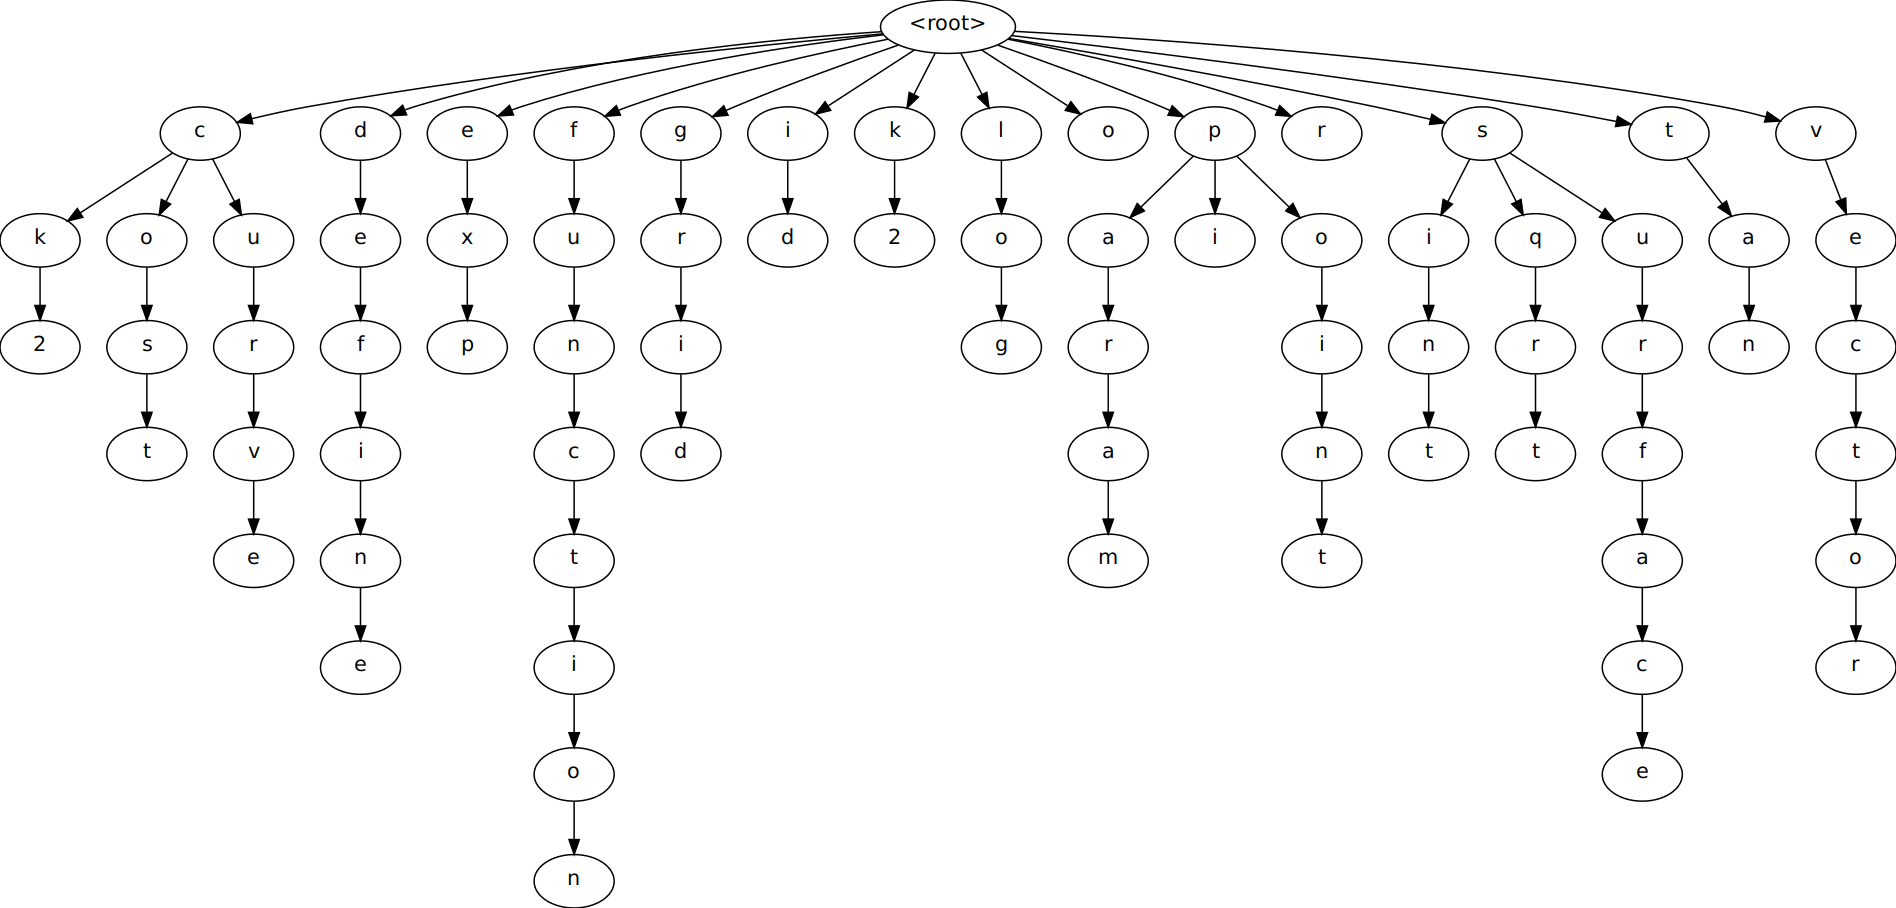
\includegraphics[width=\linewidth]{ex1table.png}
    \caption{Tabela de símbolos do exemplo 1}
    \label{img:ex1table}
\end{figure}

Nessa figura, o nó corresponente ao termo \texttt{cos} indica \texttt{type=FUNCTION},
e para \texttt{k2}, \texttt{type=CONSTANT}.

\section{Análise sintática}
A análise sintática tem a função de identificar as estruturas sintáticas
presentes nos tokens gerados pelo lexer.
O gerador, no estágio seguinte, atribui um significado para as estruturas
sintáticas reconhecidas, gerando as estruturas de dados desejadas.
O analisador sintático é chamado de parser.

\newpage
A gramática livre de contexto (\ref{grammar}) define as
regras gramaticais da linguagem.
\begin{lstlisting}[caption=Gramática livre de contexto, label=grammar]
PROG    = DECL PROG | ;

DECL    = "param"     id ":" INTS ";" ;
DECL    = "grid"      id ":" GRIDS ";" ;
DECL    = "define"    id "=" EXPR ";" ;
DECL    = "curve"     FDECL "," TINTS ";" ;
DECL    = "surface"   FDECL "," TINTS ";" ;
DECL    = "function"  FDECL ";" ;
DECL    = "point"     id "=" EXPR ";" ;
DECL    = "vector"    id "=" EXPR "@" EXPR ";" ;

FDECL   = id "(" IDS ")" "=" EXPR ;
IDS     = IDS "," id | id ;
INT     = "[" EXPR "," EXPR "]" ;
GRID    = "[" EXPR "," EXPR "," EXPR "]" ;
TINT    = id ":" INT | id ":" GRID ;
INTS    = INTS "," INT | INT ;
TINTS   = TINTS "," TINT | TINT ;
GRIDS   = GRIDS "," GRID | GRID ;

EXPR    = ADD ;
ADD     = ADD "+" JUX | ADD "-" JUX | JUX ;
JUX     = JUX MULT2 | MULT ;
MULT    = MULT "*" UNARY | MULT "/" UNARY | UNARY ;
MULT2   = MULT2 "*" UNARY | MULT2 "/" UNARY | APP ;
UNARY   = "+" UNARY | "-" UNARY | "*" UNARY | "/" UNARY | APP;
APP     = FUNC UNARY | POW ;
FUNC    = FUNC2 "^" UNARY | FUNC2 ;
FUNC2   = FUNC2 "_" var | FUNC2 "'" | func ;

POW     = COMP "^" UNARY | COMP ;
COMP    = COMP "_" num | FACT ;
FACT    = const | num | var
        | "(" TUPLE ")" | "[" TUPLE "]" | "{" TUPLE "}" ;
TUPLE   = ADD "," TUPLE | ADD ;
\end{lstlisting}

A gramática consiste em diversas igualdades.
Os termos que aparecem no lado esquerdo de alguma igualdade
são chamados de não-terminais,
e representam um conjunto de sentenças(uma sentença é uma sequência de terminais).
Os outros termos, como \texttt{";"} e \texttt{id}, são terminais,
e correspondem a tokens. Os termos \texttt{id}, \texttt{var},
\texttt{const}, \texttt{num}
e \texttt{func} representam qualquer token do tipo indicado:
\texttt{UNDEFINED}, \texttt{VARIABLE}, \texttt{CONSTANT},
\texttt{NUMBER} e \texttt{FUNCTION} respectivamente.
Os termos \texttt{"param"}, \texttt{"grid"}, \texttt{"define"}, etc.
representam os tokens do tipo \texttt{DECLARE}, que são os tipos de objeto.

Uma igualdade na gramática é dita uma produção para o não-terminal à esquerda.
O símbolo \texttt{"\textbar"}  abrevia uma produção alternativa. 
Por exemplo: \texttt{ADD = ADD + JUX | ADD - JUX | JUX}
é uma abreviação de \texttt{ADD = ADD + JUX},
\texttt{ADD = ADD - JUX} e \texttt{ADD = JUX}.
Uma produção pode ser a string vazia, por exemplo: \texttt{PROG = DECL PROG | ;}
(o ponto e vírgula no final das igualdades pertence à meta-linguagem).

Uma produção significa que o não-terminal à esquerda pode ser substituído
pela forma sentencial à direita.
Uma forma sentencial é uma sequência de terminais e não-terminais.
Por exemplo, \texttt{ADD} pode ser substituído por \texttt{ADD + JUX}.
Nesse caso, \texttt{ADD} deriva \texttt{ADD + JUX}.
Para se obter um programa gramaticalmente válido,
o não-terminal inicial \texttt{PROG} deve ser derivado até se obter somente terminais.
Uma gramática é dita ambígua quando existe uma sentença com mais de uma forma de
obtê-la a partir do não-terminal inicial.

A gramática (\ref{grammar}) não é ambígua.
A verificação foi feita em \cite{GramCheck}.
Algumas transformações na gramática a fizeram ser uma gramática LL(1).
Uma consequência disso é a não ambiguidade.
Em uma iteração anterior da gramática, a potenciação de funções
era associativa à esquerda,
enquanto a potenciação de números era à direita.
Isso causou uma ambiguidade que não foi detectada no momento.
Ela só foi descoberta ao tentar verificar a propriedade LL(1), que falhou.

O trabalho do parser, então, é achar uma forma de derivar uma
sentença a partir de \texttt{PROG}.
O método mais simples de parsing se aplica a gramáticas LL(1).

Num parser LL(1), cada não-terminal possui sua própria subrotina.
As subrotinas simulam a substituição de seu não-terminal
por uma de suas formas sentenciais possíveis.
Ou seja, uma subrotina simula uma produção de seu não-terminal.
Para decidir qual produção aplicar, as subrotinas devem consultar o token atual.
O fato da gramática ser LL(1) garante que o token atual fornece
informação suficiente para determinar qual é a produção correta e,
na falta de produção adequada,
detectar um erro gramatical. Após decidir a produção,
a subrotina começa sua simulação.
Os termos da forma sentencial da produção são tratados da esquerda para a direita.
Terminais são comparados com o token atual e um erro é detectado quando diferem.
Quando são iguais, o lexer avança para o próximo token.
Os não-terminais são substituídos imediatamente, através de suas subrotinas.

Por exemplo, considere a produção \texttt{FUNC = FUNC2 \textasciicircum UNARY}.
Para simulá-la, deve-se derivar \texttt{FUNC2}, chamando sua subrotina.
Após a subrotina terminar, o token atual é comparado com \texttt{\textasciicircum},
e caso seja igual, o lexer avança para o próximo token.
Em seguida, a subrotina \texttt{UNARY} é chamada.
No final de uma subrotina, seu não-terminal derivou uma sub-sentença,
e o token atual ficou imediatamente à direita dessa sub-sentença.
Assim, indutivamente, a rotina para \texttt{FUNC2} avançou
o token para \texttt{\textasciicircum} na produção examinada.

O termo \texttt{EXPR} define como funcionam as expressões matemáticas,
definindo operações, ordens de precedência e associatividades.
A gramática para as expressões matemáticas foi baseada na linguagem C \cite{CGram}.
Para a estética das expressões ser mais agradável, a multiplicação pode ser
por justaposição, por exemplo: \texttt{3*x = 3x}.
Em notação matemática comum, isso deixa as fórmulas muito mais simples de ler.
Vários ambientes computacionais não possuem essa facilidade,
como o Matlab, Scilab, e linguagens de programação geral.
Além disso, a aplicação de função não precisa
necessariamente de parênteses: \texttt{f(x) = fx}.
Entretanto, deve-se tomar cuidado para entender
quando que parênteses são necessários.
O fato dessa linguagem ser de domínio bem específico facilita essas decisões.

A tabela \ref{order} descreve as operações e suas ordens de precedência,
com base na gramática.

\begin{table}[ht]
\caption{Ordem das operações}
\label{order}
\begin{centering}
\begin{tabularx}{\textwidth}{||c|c|c|c|X||}
    \cline{1-5}
    Operações & Aridade & Associatividade & Exemplo & Descrição \\ \hline \hline

    \texttt{() [] \{\}} & Unário &  & \texttt{(expr)} & Isola a expressão interna \\ \hline

    , & Binário & Esquerda & \texttt{(a,b,c)} & Adiciona uma elemento à tupla(dentro de parênteses) \\ \hline

    + - & Binário & Esquerda & \texttt{a+b} & Soma e subtração \\ \hline

    \textit{justaposição} & Binário & Esquerda & \texttt{ab} & Multiplicação justaposta \\ \hline

    * / & Binário & Esquerda & \texttt{a*b} & Multiplicação e Divisão \\ \hline

    + - * / & Unário &  & \texttt{-x}, \texttt{*v} & Positivo, Negativo, Quadrado e Recíproco \\ \hline

    \textit{aplicação} & Binário & Esquerda & \texttt{sin x} & Aplicação de função \\ \hline

    \textasciicircum & Binário & Direita & \texttt{a\textasciicircum b} & Potenciação \\ \hline

    \_ & Unário & & \texttt{(1, 2, 3)\_2} & Elemento de tupla \\ \hline
    
    ' \_ & Unário & & \texttt{sin'x + f\_z(3)} & Derivada Total e Parcial \\ \hline
    \cline{1-5}
\end{tabularx}
\end{centering}
\end{table}

\newpage
A estrutura \texttt{Parser} (\ref{parser}) define o parser.

\begin{lstlisting}[caption=Estrutura parcial do parser, label=parser]
struct Parser
{
    Lexer lexer;
    std::unique_ptr<Table> table = std::make_unique<Table>();
    std::vector<std::vector<Table*>> argList;
    Table *objType{};
    Table *objName{};
    Table *tag{};
    int tupleSize = 0;

    #define INIT(x, y) Table *x = table->initString(#x, TokenType::y);
        INIT(param,     DECLARE)
        INIT(pi,        CONSTANT)
        INIT(sqrt,      FUNCTION)
        /*.....*/
    #undef INIT

    Parser();
    void advance(bool match = true);

    typedef void Parse();

    void parseProgram(const char *source);

    Parse 
        parseFDecl, parseParam, parseGrid, parseDefine /*.....*/;

    void parseInt(ExprType type);
    void parseInts(ExprType type);

    void parseMult(bool unary);

    virtual void actAdvance();
    virtual void actInt(ExprType type);
    virtual void actOp(ExprType type);
    virtual void actDecl();

    virtual ~Parser() = 0;
};
\end{lstlisting}

O membro \texttt{lexer} é o analisador léxico.
O parser controla o avanço dos tokens diretamente.
O membro \texttt{table} é a tabela de símbolos compartilhada
pelos estágios da compilação.
O membro \texttt{argList} é uma lista de listas identificadores.
O atributo \texttt{argIndex} de um token de função é um índice dessa lista,
indicando a lista de parâmetros da função(exceto para as funções pré-definidas).
Os membros \texttt{objType} e \texttt{objName} auxiliam o estágio da geração,
e correspondem ao tipo de objeto e seu nome.
O membro \texttt{tag} é o nome do argumento marcado em um intervalo do tipo tag.
Os membros \texttt{param}, \texttt{pi}, \texttt{sqrt}, etc. são
as palavras-chave, funções e constantes pré-definidas.

Os métodos com prefixo \texttt{parse} são as subrotinas dos não-terminais.
A lógica do código foi simplificada, então não há uma correspondência exata.
Os métodos com prefixo \texttt{act}, marcados com \texttt{virtual},
são implementados no estágio seguinte.
Esses métodos são chamados de ações semânticas,
e são invocados pelo parser quando uma estrutura sintática é detectada.

O método \texttt{advance} chama \texttt{actAdvance} e avança o token.
Isso possibilita uma reação a um comentário ou a um token qualquer.
O compilador não usa essa ação semântica.
Essa ação semântica é usada no \textit{syntax highlighting},
uma outro ``compilador'', que serve para atribuir cores ao texto do programa.
As cores são determinadas conforme o tipo de token e conforme uma 
paleta pré-definida.
Desse modo, um comentário pode ser colorido pois não é exatamente ignorado.

Quando uma função está sendo definida, os identificadores de seus argumentos
passam a ser do tipo \texttt{VARIABLE}.
Após a definição, são redefinidos para \texttt{UNDEFINED}.

\section{Análise semântica e síntese}
A análise semântica e síntese é responsável pela geração das estruturas de dados
adequadas para a visualização dos objetos.
A síntese é o estágio mais complexo do projeto.

Para os parâmetros, o compilador cria um controle deslizante na interface.
Para os objetos desenháveis, cria as funções para a renderização.

\newpage
A estrutura \texttt{Compiler} (\ref{compiler}) define o compilador.

\begin{lstlisting}[caption=Estrutura parcial do compilador, label=compiler]
struct Compiler : public Parser
{
    std::vector<std::unique_ptr<SymbExpr>> symbExprs;
    std::vector<std::unique_ptr<CompExpr>> compExprs;
    std::vector<SymbExpr*> expStack;
    std::vector<Interval> intStack;
    std::vector<Obj> objects;
    Size frameSize = {512, 512};

    Buffer block{};
    uint blockSize{};
    /*.....*/

    bool compiled = false;

    void actInt(ExprType type);
    void actOp(ExprType type);
    void actDecl();
    
    SymbExpr *newExpr(SymbExpr &e);
    CompExpr *newExpr(CompExpr &e);
    SymbExpr op(Parser::ExprType type, SymbExpr *a = nullptr, SymbExpr *b = nullptr, float number = 0, Table *name = nullptr);
    CompExpr *op(CompExpr::ExprType type, CompExpr *a = nullptr, CompExpr *b = nullptr, float number = 0, Table *name = nullptr, int nTuple = 1);
    CompExpr *_comp(CompExpr *e, unsigned int index, std::vector<Subst> &subs);
    CompExpr *compute(SymbExpr *e, std::vector<Subst> &subs);
    CompExpr *substitute(CompExpr *e, std::vector<Subst> &subs);
    CompExpr *derivative(CompExpr *e, Table *var);
    float calculate(CompExpr *e, std::vector<Subst> &subs);
    void dependencies(CompExpr *e, std::vector<int> &grids, bool allow = false);

    void compile(CompExpr *e, std::stringstream &str, int &v);
    void compile(const char *source);
    void header(std::stringstream &str);
    void compileFunction(CompExpr *exp, int argIndex, std::stringstream &str, std::string name);
    void declareFunction(int N, int argIndex, std::stringstream &str, std::string name, bool declareOnly = false);
};
\end{lstlisting}

Os métodos de prefixo \texttt{act} implementam as
ações semânticas invocadas pelo parser.
\texttt{actInt} é a ação mais simples e apenas junta as informações
para construír um intervalo.
\texttt{actOp} gera as árvores de expressões matemáticas.
\texttt{actDecl} junta as informações para contruír um objeto declarado.

Os métodos de \texttt{newExpr} a \texttt{dependencies} processam
as expressões matemáticas para uma forma mais tratável.
\texttt{newExpr} e \texttt{op} auxiliam na criação de expressões matemáticas, e são usadas
em vários outros métodos.
\texttt{\_comp} auxilia o acesso de um elemento de uma tupla, por exemplo:
\texttt{(x, y, z)\_1 = x}, e \texttt{p\_1 = p\_1} para uma constante \texttt{p}.
\texttt{compute} é o método principal e invoca os outros métodos, além de
descompactar algumas operações.
O método \texttt{substitute} resolve funções, substituindo uma aplicação pelo corpo da função.
O método \texttt{derivative} computa derivadas simbólicas.
O método \texttt{calculate} calcula o valor numérico de uma expressão, 
quando possível, e é usado para cálculos feitos na \textit{CPU}, pois
as expressões são compiladas apenas para a \textit{GPU}.
O método \texttt{dependencies} detecta de quais grades um objeto depende.

Os métodos de \texttt{compile} a \texttt{declareFunction} geram o produto final.
Juntos, geram os códigos-fonte na linguagem de \textit{shader}(GLSL) do OpenGL.
O método \texttt{header} auxilia a declaração dos parâmetros na linguagem GLSL.
O método \texttt{compileFunction} apenas auxilia o retorno das funções no código GLSL.
O método \texttt{declareFunction} auxilia na declaração das funções.
O primeiro método \texttt{compile} gera o código-fonte para calcular o valor de uma
expressão.
Por exemplo, a expressão matemática \texttt{x*3+1} é
compilada para(aproximadamente) o seguinte código:

\begin{lstlisting}
float v0 = x;
float v1 = 3;
float v2 = v0*v1;
float v3 = 1;
float v4 = v2+v3;
\end{lstlisting}

O código é gerado por um algoritmo na árvore da expressão,
então o código-fonte gerado pode ser bem verboso/grande.

O segundo método \texttt{compile} é o método principal.
Ele inicializa e invoca o parser.
Após o parser finalizar seu trabalho, os objetos estão descritos
numa estrutura de dados fácil de manipular.
O método então compila as expressões matemáticas, e finalmente gera o produto final.
Para os objetos desenháveis, gera as funções para desenhá-los.
Para superfícies, compila também o geodesic tracing.
Para os parâmetros, gera controles deslizantes na interface.
Ao finalizar, a interface está pronta para a interação com os objetos.

O compilador também verifica a validade semântica dos objetos.
Por exemplo, intervalos não podem depender de parâmetros ou grades.
Curvas e superfícies devem ter o número correto de parâmetros, e devem estar
definidos em 3 dimensões.

%\chapter{Desenvolvimento}

Corresponde ao corpo do trabalho, contendo a exposição ordenada e pormemorizada
do assunto. Constam aqui a revisão de literatura, metodologia adotada, os resultados e
sua discussão. Divide-se em seções e subseções. \cite{Robert2007}


%\chapter{Conclusions}
\label{ch:conclusions}




% -----------------------------------
% ELEMENTOS PÓS-TEXTUAIS
% -----------------------------------
\postextual
% ----------------------------------

%\bibliography{biblio}
\printbibliography

%\glossary

% ----------------------------------------------------------
% Apêndices
% ----------------------------------------------------------

% ---
% Inicia os apêndices
% ---
% \begin{apendicesenv}

% % Imprime uma página indicando o início dos apêndices
% \partapendices

% \end{apendicesenv}
% ---

% ----------------------------------------------------------
% Anexos
% ----------------------------------------------------------

% \begin{anexosenv}

% \partanexos

% \end{anexosenv}

%---------------------------------------------------------------------
% ÍNDICE REMISSIVO
%---------------------------------------------------------------------
\phantompart
\printindex

\end{document}